\documentclass[es,boletin]{uah}

\usepackage{subfigure}
\usepackage{amsfonts}
\usepackage{hyperref}

\tema{4}
\titulo{Teoría de la detección}{Detection theory}
%
\begin{document}

\titulacion{Grados TIC}
\asignatura{Teoría de la Comunicación}{Communication Theory}
\departamento{Teoría de la Señal y Comunicaciones}
\curso{2024/2025} % Do not show year

\maketitle
	
\seccion{Conceptos a repasar}{Key concepts}
\texto{
Antes de hacer estos ejercicios es importante repasar y tener claros los siguientes conceptos teóricos:

\begin{itemize}
\item Esquema general de un sistema de comunicaciones digital. 
\item Conceptos de base ortonormal, espacio de señal y constelación.
\item Cómo se calcula una base ortonormal a partir de un conjunto de señales transmitidas.
\item Criterios de decisión (MAP y ML). Regiones de decisión.
\item Cálculo de la probabilidad de error.
\item Cotas. Diferencias entre la cota de la unión y la cota de la unión simplificada.
\item Implementación del demodulador: banco de correladores o filtros adaptados.
\item Implementación del decisor: esquema teórico o implementación práctica.
\end{itemize}
}
{
	Before doing these exercises it is important to review and understand the following concepts:	

	\begin{itemize}
		\item General diagram of a digital communication system.
		\item Concepts of orthonormal basis, signal space and constellation.
		\item How an orthonormal basis is computed from a set of transmitted signals.
		\item Decision criteria (MAP and ML). Decision regions.
		\item Calculation of the probability of error.
		\item Bounds. Differences between the union bound and the simplified union bound.
		\item Demodulator implementation: bank of correlators or matched filters.
		\item Decisor implementation: theoretical scheme or practical implementation.
	\end{itemize}
}

%%%%%%%%%%%%%%%%%%%%%%%%%%%%%%%%%%%%%%%%%%%%%%%%%%%%%%%%
%%%%%%%%%%%%%%%%%%%%%%%%%%%%%%%%%%%%%%%%%%%%%%%%%%%%%%%%
\seccion{Problemas básicos}{Basic problems}
%%%%%%%%%%%%%%%%%%%%%%%%%%%%%%%%%%%%%%%%%%%%%%%%%%%%%%%%
%%%%%%%%%%%%%%%%%%%%%%%%%%%%%%%%%%%%%%%%%%%%%%%%%%%%%%%%
\texto{
	Este primer bloque de problemas son problemas extraídos en su mayoría de la bibliografía de la asignatura, y consisten en algunos cálculos básicos que es necesario dominar.

}
{
	This first part includes problems mostly extracted from the bibliography aimed at practicing basic calculations needed for the rest of the lesson.

}



\Problema{
	\cite{Artes} Considere la constelación de señales $\{s_i(t), i=0,\cdots , M-1\}$, idénticamente nula fuera del intervalo $0\leq t<T$, y de valor 
	\begin{displaymath}
		s_i(t) = \sen\left ( \frac{2\pi(i+1)t}{T} \right )
	\end{displaymath}
	dentro de este. Determine una base ortonormal para representar la constelación de señales, sus coordenadas con respecto a esta base, la distancia entre cualesquiera dos señales, la energía de cada señal de la constelación y la energía media de la constelación.
}
{
	\begin{enumerate}
		\item $\phi_i(t) = \sqrt{\frac{2}{T}} \sen\left ( \frac{2\pi(i+1)t}{T} \right )$
 	 	\item $d_{ij} = \sqrt{T}$
    	\item $Ei = E_s = \frac{T}{2}$	
	\end{enumerate}
}
{
	\cite{Artes} Consider the constellation of signals $\{s_i(t), i=0,\cdots , M-1\}$, identically null outside the interval $0\leq t<T$, and of value
	\begin{displaymath}
	s_i(t) = \sin\left ( \frac{2\pi(i+1)t}{T} \right )
	\end{displaymath}
	inside it. Determine an orthonormal basis to represent the constellation of signals, its coordinates with respect to this basis, the distance between any two signals, the energy of each signal in the constellation, and the mean energy of the constellation.
}
{
	\begin{enumerate}
		\item $\phi_i(t) = \sqrt{\frac{2}{T}} \sen\left ( \frac{2\pi(i+1)t}{T} \right )$
 	 	\item $d_{ij} = \sqrt{T}$
    	\item $Ei = E_s = \frac{T}{2}$	
	\end{enumerate}
}


\Problema{
	\cite{Sklar} Determina si $s_1(t)$ y $s_2(t)$ son ortogonales en el intervalo $(-1.5T<t<1.5T)$, donde $s_1(t) = \cos(\omega_1 t + \phi_1)$, $s_2(t) = \cos(\omega_2 t + \phi_2)$, y $\omega_2 = 2\pi/T$ para los siguientes casos:

	\begin{enumerate}
		\item $\omega_1 = \omega_2$ y $\phi_1 = \phi_2$
  		\item $\omega_1 = 2 \omega_2$ y $\phi_1 = \phi_2$
    	\item $\omega_1 = \omega_2$ y $\phi_1 = \phi_2 + \pi/2$
     	\item $\omega_1 = \omega_2$ y $\phi_1 = \phi_2 + \pi$
	\end{enumerate}
}
{
	\begin{enumerate}
		\item No son ortogonales.
  		\item Sí son ortogonales.
    	\item Sí son ortogonales
     	\item No son ortogonales
	\end{enumerate}
}
{
	\cite{Sklar} Determine whether or not $s_1(t)$ and $s_2(t)$ are orthogonal over the interval $(-1.5T<t<1.5T)$, where $s_1(t) = \cos(\omega_1 t + \phi_1)$, $s_2(t) = \cos(\omega_2 t + \phi_2)$, and $\omega_2 = 2\pi/T$ for the following cases:

	\begin{enumerate}
		\item $\omega_1 = \omega_2$ and $\phi_1 = \phi_2$
  		\item $\omega_1 = 2 \omega_2$ and $\phi_1 = \phi_2$
    	\item $\omega_1 = \omega_2$ and $\phi_1 = \phi_2 + \pi/2$
     	\item $\omega_1 = \omega_2$ and $\phi_1 = \phi_2 + \pi$
	\end{enumerate}
}
{
	\begin{enumerate}
		\item Not orthogonal
  		\item Orthogonal
    	\item Orthogonal
     	\item Not orthogonal
	\end{enumerate}
}

%%%%%%%%%%%%%
% PROBLEMA 1
%%%%%%%%%%%%%
\Problema{

	Dadas las constelaciones de señales equiprobables, mostradas en la siguiente figura, se pide calcular los apartados a y b de todas ellas:
	
	\begin{enumerate}
		\item El valor de A para que $E_s=1 J$.
		\item Establecer las regiones de decisión, así como una cota de la probabilidad de error, $P_e$, con $N_0/2=-13 dBW/Hz$.
	\end{enumerate}



	{\begin{figure*}[h!]\centering
	\begin{subfigure}{}
	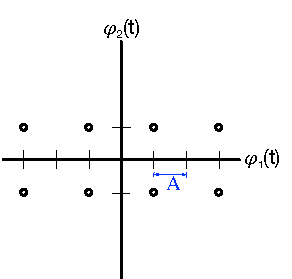
\includegraphics[width=3cm]{./Figuras/Problema4_1a}
	\end{subfigure}
	\begin{subfigure}{}
	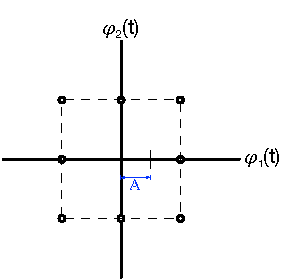
\includegraphics[width=3cm]{./Figuras/Problema4_1b}
	\end{subfigure} \\
	\begin{subfigure}{}
	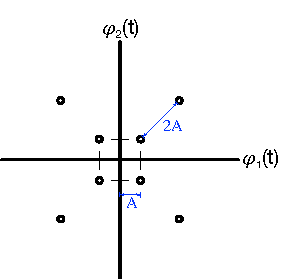
\includegraphics[width=3cm]{./Figuras/Problema4_1c}
	\end{subfigure}
	\begin{subfigure}{}
	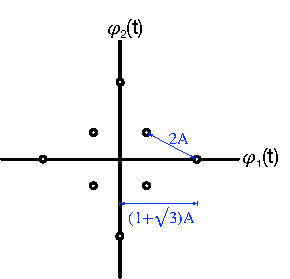
\includegraphics[width=3cm]{./Figuras/Problema4_1d}
	\end{subfigure}
	\end{figure*}}

}
{
\begin{enumerate}
	\item $A=\frac{1}{\sqrt{6}}$, $A=\frac{1}{\sqrt{6}}$, $A=\frac{1}{\sqrt{2 (2 + \sqrt{2})}}$, $A=\sqrt{\frac{2}{11}}$
	\item $P_e = 0.2515$, $P_e = 0.2515$, $P_e = 0.31199$, $P_e = 0.2010$
\end{enumerate}

	{\begin{figure}[h!]\centering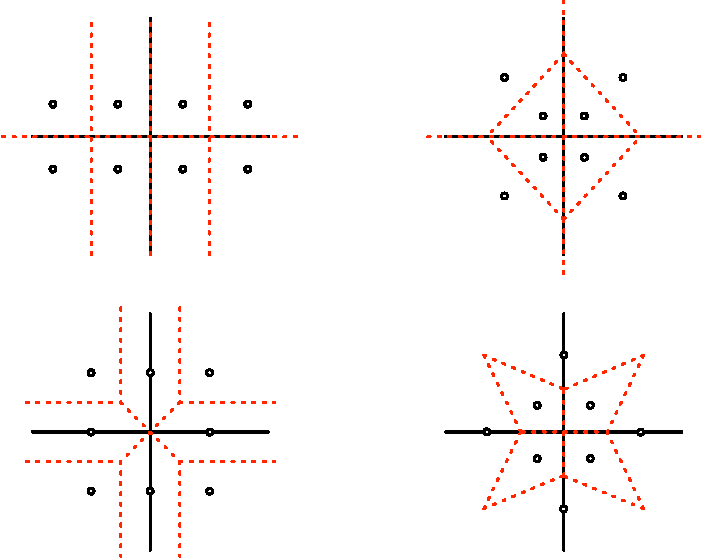
\includegraphics[width=6cm]{./Figuras/Problema4_1_sol}\end{figure}}
}		
{

	Consider the constellations plotted below, where the signals are equiprobable. For each of them, calculate a. and b.:
	
	\begin{enumerate}
		\item The value of the constant $A$ so that $E_s=1 J.$
		\item The decision regions and a bound on the probability of error for $N_0/2=-13 dBW/Hz$.
	\end{enumerate}

	{\begin{figure*}[h!]\centering
	\begin{subfigure}{}
	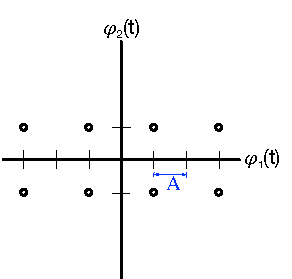
\includegraphics[width=3cm]{./Figuras/Problema4_1a}
	\end{subfigure}
	\begin{subfigure}{}
	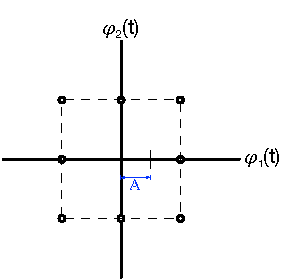
\includegraphics[width=3cm]{./Figuras/Problema4_1b}
	\end{subfigure} \\
	\begin{subfigure}{}
	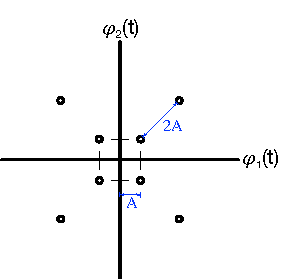
\includegraphics[width=3cm]{./Figuras/Problema4_1c}
	\end{subfigure}
	\begin{subfigure}{}
	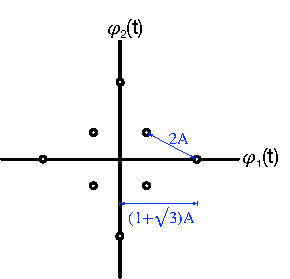
\includegraphics[width=3cm]{./Figuras/Problema4_1d}
	\end{subfigure}
	\end{figure*}}

}
{
\begin{enumerate}
	\item $A=\frac{1}{\sqrt{6}}$, $A=\frac{1}{\sqrt{6}}$, $A=\frac{1}{\sqrt{2 (2 + \sqrt{2})}}$, $A=\sqrt{\frac{2}{11}}$
	\item $P_e = 0.2515$, $P_e = 0.2515$, $P_e = 0.31199$, $P_e = 0.2010$
\end{enumerate}


	{\begin{figure}[h!]\centering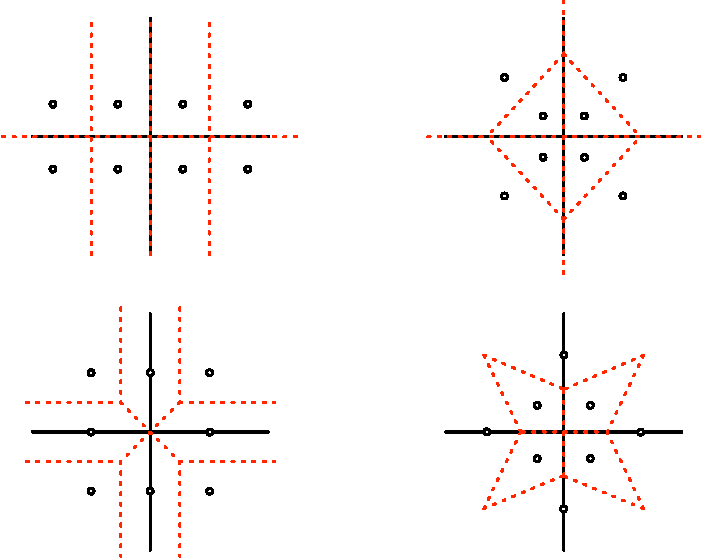
\includegraphics[width=6cm]{./Figuras/Problema4_1_sol}\end{figure}}
}		

%%%%%%%%%%%%%
% PROBLEMA 2
%%%%%%%%%%%%%
\Problema{

	Dado el siguiente conjunto de señales, definidas en el intervalo $-1\leq t<1$:
	
	\begin{displaymath}
		s_1 (t)=1 
	\end{displaymath}
	\begin{displaymath}
		s_2(t) = t
	\end{displaymath}
	\begin{displaymath}
		s_3(t) = t^2
	\end{displaymath}

Se pide:

\begin{enumerate}
	\item Utilizando el método de Gram-Schmidt, encontrar una base ortonormal que permita representar las señales.
	\item Representar la constelación correspondiente.
\end{enumerate}

}
{
\begin{enumerate}
	\item $\phi_1(t) = \frac{1}{\sqrt{2}}$ ; $-1 \leq t < 1$\\
	 $\phi_2(t) = \sqrt{\frac{3}{2}}t$; $-1 \leq t < 1$\\
	 $\phi_3(t) = \sqrt{\frac{45}{8}}\left ( t^2 - \frac{1}{3}\right )$, $-1 \leq t < 1$
	\item $s_1(t) = \sqrt{2}\cdot \phi_1(t)$\\
		 $s_2(t)=\sqrt{\frac{2}{3}} \cdot \phi_2(t)$\\
		  $s_3(t) = \frac{\sqrt{2}}{3}\cdot \phi_1(t) + \sqrt{\frac{8}{45}} \cdot \phi_3(t)$
\end{enumerate}
}
{

	Consider the following signal set, defined within the interval $-1 \leq t < 1$.

	\begin{displaymath}
		s_1 (t)=1 
	\end{displaymath}
	\begin{displaymath}
		s_2(t) = t
	\end{displaymath}
	\begin{displaymath}
		s_3(t) = t^2
	\end{displaymath}

Calculate:

\begin{enumerate}
	\item An orthonormal basis to represent said signal set, by using the Gram-Schmidt method.
	\item Plot the corresponding constellation.
\end{enumerate}

}
{
\begin{enumerate}
	\item $\phi_1(t) = \frac{1}{\sqrt{2}}$ ; $-1 \leq t < 1$\\
	 $\phi_2(t) = \sqrt{\frac{3}{2}}t$; $-1 \leq t < 1$\\
	 $\phi_3(t) = \sqrt{\frac{45}{8}}\left ( t^2 - \frac{1}{3}\right )$, $-1 \leq t < 1$
	\item $s_1(t) = \sqrt{2}\cdot \phi_1(t)$\\
		 $s_2(t)=\sqrt{\frac{2}{3}} \cdot \phi_2(t)$\\
		  $s_3(t) = \frac{\sqrt{2}}{3}\cdot \phi_1(t) + \sqrt{\frac{8}{45}} \cdot \phi_3(t)$
\end{enumerate}
}


%%%%%%%%%%%%%
% PROBLEMA 3
%%%%%%%%%%%%%
\Problema{

Para transmitir un conjunto de ocho símbolos equiprobables a través de un sistema en banda base, se eligen las ocho señales representadas en la figura. 

{\begin{figure*}[h!]\centering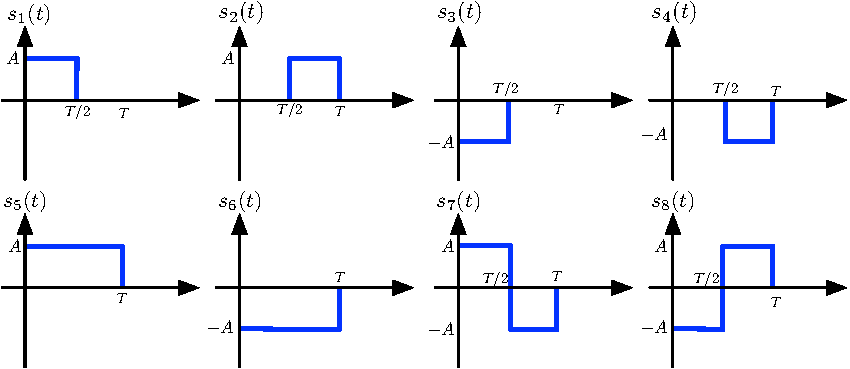
\includegraphics[width=12cm]{./Figuras/Problema4_3}\end{figure*}}


\begin{enumerate}
	\item Dibujar una posible constelación del conjunto de señales, indicando la distancia entre las señales adyacentes.
\end{enumerate}

}
{
\begin{enumerate}
	\item $d_{12} = d_{14} = A \cdot \sqrt{T}$, $d_{13} = A \cdot \sqrt{2T}$, $d_{15}=d_{17} = A \cdot \sqrt{\frac{T}{2}}$, $d_{16}=d_{18} = A \cdot \sqrt{\frac{5T}{2}}$
	 
{\begin{figure*}[h!]\centering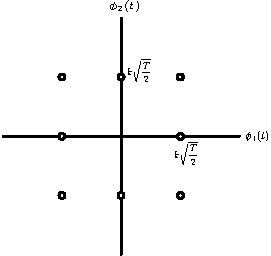
\includegraphics[width=4cm]{./Figuras/Problema4_3_sol}\end{figure*}}

\end{enumerate}
}
{

In order to transmit a set of eight equiprobable symbols by means of a baseband system, the eight signals in the figure are chosen.


{\begin{figure*}[h!]\centering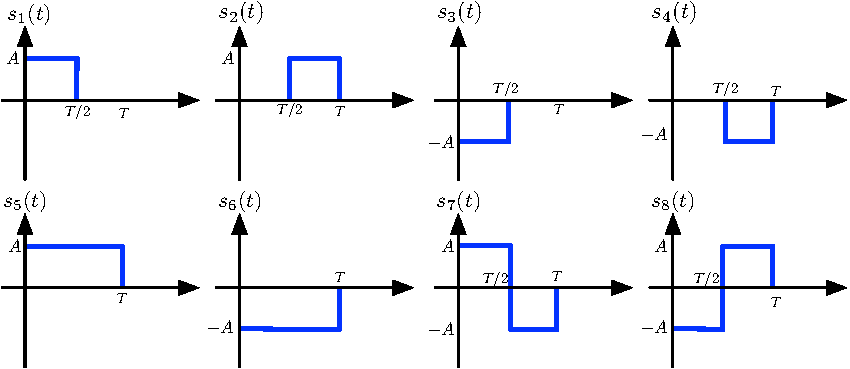
\includegraphics[width=12cm]{./Figuras/Problema4_3}\end{figure*}}


\begin{enumerate}
	\item Depict a possible constellation for this signal set and give the distance between adjacent signals.
\end{enumerate}

}
{
\begin{enumerate}
	\item $d_{12} = d_{14} = A \cdot \sqrt{T}$, $d_{13} = A\cdot \sqrt{2T}$, $d_{15}=d_{17} = A \cdot \sqrt{\frac{T}{2}}$, $d_{16}=d_{18} = A \cdot \sqrt{\frac{5T}{2}}$
	 
{\begin{figure*}[h!]\centering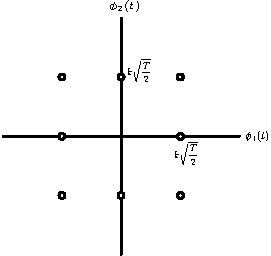
\includegraphics[width=4cm]{./Figuras/Problema4_3_sol}\end{figure*}}

\end{enumerate}
}

%%%%%%%%%%%%%
% PROBLEMA 4
%%%%%%%%%%%%%
\Problema{

	Se utilizan las señales de la siguiente figura, para transmitir dos mensajes equiprobables, a través de un canal perturbado por ruido aditivo blanco Gaussiano, con densidad espectral de potencia de ruido $N_0/2=1W/Hz$.
	
	{\begin{figure*}[h!]\centering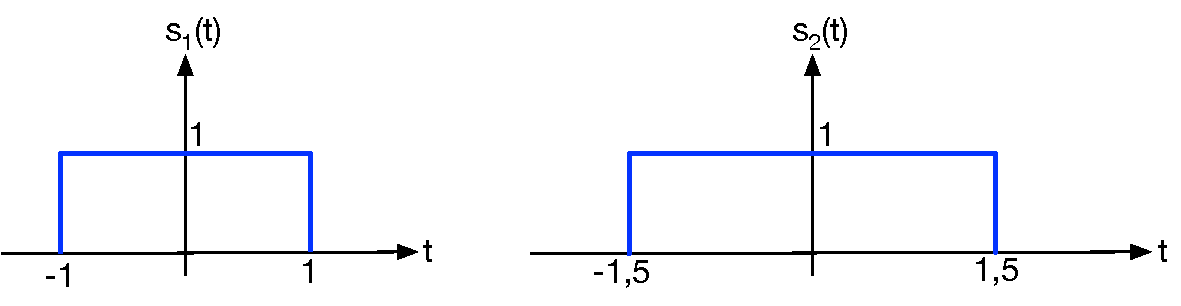
\includegraphics[width=10cm]{./Figuras/Problema4_4}\end{figure*}}
	Se pide:
	
	\begin{enumerate}
		\item Obtener y representar una base ortonormal que permita representar la constelación de las dos señales.
		\item Representar la constelación correspondiente.
		\item Calcular la probabilidad de error correspondiente.
	\end{enumerate}

}
{
\begin{enumerate}
	\item \ \\ 
	$\begin{array}{ll}
			\phi_1(t) = \frac{1}{\sqrt{2}} s_1(t) & -1\leq t<1 \\
			\phi_2(t) = s_2(t) - s_1(t)		& -1.5 \leq t < 1,5\\
			\end{array}$
	\item $s_1(t) = \sqrt{2} \phi_1(t)$, $s_2(t) = \sqrt{2}\phi_1(t) + \phi_2(t)$
	
		{\begin{figure*}[h!]\centering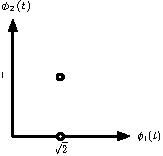
\includegraphics[width=4cm]{./Figuras/Problema4_4_sol}\end{figure*}}
	\item $P_e = Q(0.5) = 0.30853$
\end{enumerate}
}
{

	The signals depicted below are used to transmit two possible equiprobable messages across a channel distorted by AWGN, whose power density spectrum is $N_0/2=1W/Hz$.
	
	{\begin{figure*}[h!]\centering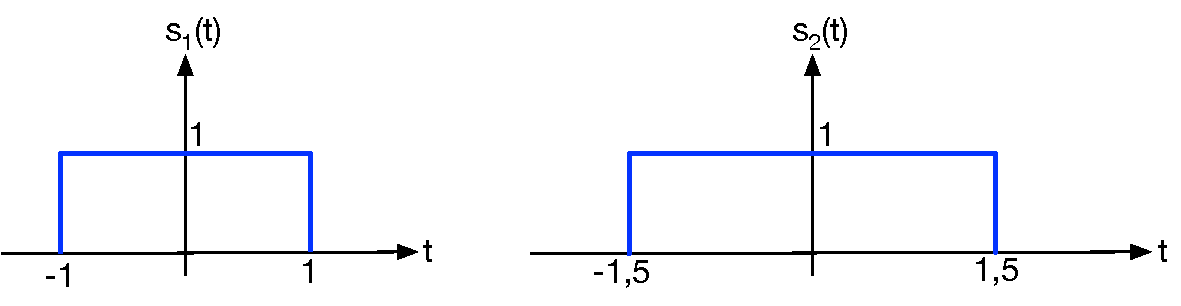
\includegraphics[width=10cm]{./Figuras/Problema4_4}\end{figure*}}
	
	\begin{enumerate}
		\item Calculate and plot an orthonormal basis for this signal set.
		\item Plot the corresponding constellation.
		\item Calculate the corresponding error probability.
	\end{enumerate}

}
{
\begin{enumerate}
	\item \ \\ 
	 $\begin{array}{ll}
			\phi_1(t) = \frac{1}{\sqrt{2}} s_1(t) & -1\leq t<1 \\
			\phi_2(t) = s_2(t) - s_1(t)		& -1.5 \leq t < 1,5\\
			\end{array}$
	\item $s_1(t) = \sqrt{2} \phi_1(t)$, $s_2(t) = \sqrt{2}\phi_1(t) + \phi_2(t)$
	
		{\begin{figure*}[h!]\centering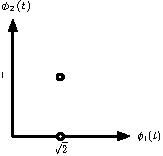
\includegraphics[width=4cm]{./Figuras/Problema4_4_sol}\end{figure*}}
	\item $P_e = Q(0.5) = 0.30853$
\end{enumerate}
}


%%%%%%%%%%%%%
% PROBLEMA 9
%%%%%%%%%%%%%
\Problema{

Sea el conjunto de señales dado por la expresión:
	
	\begin{displaymath}
		s_i(t) = \left \{ 
		\begin{array}{ll}
		\sqrt{\frac{2E}{T}} cos \left (\omega_c t + i \frac{\pi}{4} \right ) & 0 \leq t < T \\
		0 & c.c.
		\end{array}
		\right.
	\end{displaymath}

donde $i=1,2,3,4$ y $\omega_c  = n_c\cdot \frac{2\pi}{T}$ para algún valor entero $n_c$.

\begin{enumerate}
	\item ¿Cuál es la dimensión, $N$, del espacio generado por este conjunto de señales?
	\item Obtenga una base ortonormal para representar este conjunto.
	\item Obtenga los vectores de señal de cada una de las señales $s_i(t)$.
	\item Dibuje los vectores de señal en el espacio de señal.
\end{enumerate}

}
{

\begin{enumerate}
	\item $N=2$
	\item \
	\begin{displaymath}
		\begin{array}{ll}
			\phi_1(t) = \sqrt{\frac{2}{T}} cos \left ( \omega_c t + \frac{\pi}{4} \right ) & 0 \leq t < T \\
			\phi_2(t) = \sqrt{\frac{2}{T}} cos \left ( \omega_c t + \frac{3\pi}{4} \right ) & 0 \leq t < T \\
		\end{array}
	\end{displaymath}
	\item \
	\begin{displaymath}
		\begin{array}{ll}
			\bar{s_1} = \left [\sqrt{E}, 0 \right ] & \bar{s_2} = \left [\sqrt{\frac{E}{2}}, \sqrt{\frac{E}{2}} \right ] \\
			\bar{s_3} = \left [0, \sqrt{E} \right ] & \bar{s_4} = \left [-\sqrt{\frac{E}{2}}, \sqrt{\frac{E}{2}} \right ]\\
		\end{array}
	\end{displaymath}
	\item \
	\begin{figure*}[h!] 	\centering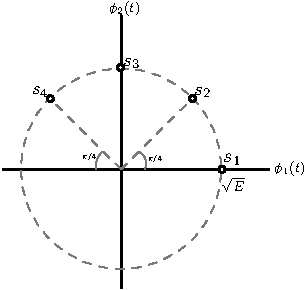
\includegraphics[width=4cm]{./Figuras/Problema4_9_sol} 	\end{figure*}
\end{enumerate}

}
{

	Consider the signal set given by:
	
	\begin{displaymath}
		s_i(t) = \left \{ 
		\begin{array}{ll}
		\sqrt{\frac{2E}{T}} cos \left (\omega_c t + i \frac{\pi}{4} \right ) & 0 \leq t < T \\
		0 & c.c.
		\end{array}
		\right.
	\end{displaymath}

where $i=1,2,3,4$ and $\omega_c  = n_c\cdot \frac{2\pi}{T}$ for some integer value $n_c$.

\begin{enumerate}
	\item Which is the dimension, $N$, of the space generated by this signal set?
	\item Obtain an orthonormal basis for this set.
	\item Obtain the signal vectors for each of the signals $s_i(t)$.
	\item Plot the signal vectors in the signal space.
\end{enumerate}
	
}
{

\begin{enumerate}
	\item $N=2$
	\item \
	\begin{displaymath}
		\begin{array}{ll}
			\phi_1(t) = \sqrt{\frac{2}{T}} cos \left ( \omega_c t + \frac{\pi}{4} \right ) & 0 \leq t < T \\
			\phi_2(t) = \sqrt{\frac{2}{T}} cos \left ( \omega_c t + \frac{3\pi}{4} \right ) & 0 \leq t < T \\
		\end{array}
	\end{displaymath}
	\item \
	\begin{displaymath}
		\begin{array}{ll}
			\bar{s_1} = \left [\sqrt{E}, 0 \right ] & \bar{s_2} = \left [\sqrt{\frac{E}{2}}, \sqrt{\frac{E}{2}} \right ] \\
			\bar{s_3} = \left [0, \sqrt{E} \right ] & \bar{s_4} = \left [-\sqrt{\frac{E}{2}}, \sqrt{\frac{E}{2}} \right ]\\
		\end{array}
	\end{displaymath}
	\item \
	\begin{figure*}[h!] 	\centering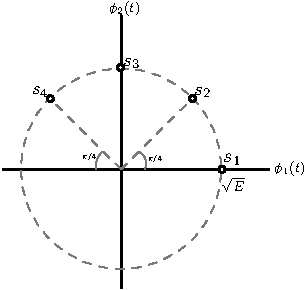
\includegraphics[width=5cm]{./Figuras/Problema4_9_sol} 	\end{figure*}
\end{enumerate}

}

%%%%%%%%%%%%%
% PROBLEMA 12
%%%%%%%%%%%%%
\Problema{

	Se dispone de un sistema de transmisión digital que transmite los símbolos $0$ y $A$. A la entrada del receptor el ruido es aditivo, blanco y gaussiano, con densidad espectral de potencia $N_0/2 = 0.01 W/Hz$. Calcular la amplitud con que deben ser recibidos para garantizar que solo uno de cada millón de bits enviados sea recibido erróneamente.
}
{

$A > 0.96$

}
{

	A digital transmission system transmits the symbols $0$ and $A$. At the receiver, the noise can be considered as white and Gaussian, with power spectral density $N_0/2 = 0.01 W/Hz$. If we suppose rectangular pulses, calculate the amplitude at the transmitter to guarantee that only $1$ out of $10^6$ bits is wrongly received.
	
}
{

$A > 0.96$

}

%%%%%%%%%%%%%
% PROBLEMA 13
%%%%%%%%%%%%%
\Problema{

	Sea un sistema de transmisión digital con dígitos equiprobables $0$ y $A$, y $\left ( \frac{S}{N} \right )_R=50$. 
	
	Calcule las probabilidades de error $P_{e|0}$ (probabilidad de error condicionada a que se ha transmitido el símbolo 0), $P_{e|A}$ y $P_e$ cuando el umbral se sitúa en el valor $V=0.4 A$ y compárelo con el mínimo dado por la ecuación $P_e=Q\left ( \frac{A}{2\sigma} \right )$.
}
{

\begin{itemize}
	\item $P_{e|0} = Q(4)$
	\item $P_{e|A} = Q(6)$
	\item $P_e = 1.58 \cdot 10^{-5}$
	\item $P_{e_{min}} = 2.87 \cdot 10^{-7}$
\end{itemize}
}
{

	Consider a digital system with equiprobable digits $0$ and $A$, and $\left ( \frac{S}{N} \right )_R=50$. 
	
	
	Calculate the error probabilities $P_{e|0}$ (error probability conditioned to the transmission of symbol 0), $P_{e|A}$ and $P_e$ when the threshold is situated in $V=0.4 A$, and compare it when the minimum given by the equation $P_e=Q\left ( \frac{A}{2\sigma} \right )$.
}
{

\begin{itemize}
	\item $P_{e|0} = Q(4)$
	\item $P_{e|1} = Q(6)$
	\item $P_e = 1.58 \cdot 10^{-5}$
	\item $P_{e_{min}} = 2.87 \cdot 10^{-7}$
\end{itemize}
}








%%%%%%%%%%%%%%%%%%%%%%%%%%%%%%%%%%%%%%%%%%%%%%%%%%%%%%%%
%%%%%%%%%%%%%%%%%%%%%%%%%%%%%%%%%%%%%%%%%%%%%%%%%%%%%%%%
\newpage
\seccion{Problemas adicionales}{Aditional problems}
%%%%%%%%%%%%%%%%%%%%%%%%%%%%%%%%%%%%%%%%%%%%%%%%%%%%%%%%
%%%%%%%%%%%%%%%%%%%%%%%%%%%%%%%%%%%%%%%%%%%%%%%%%%%%%%%%
\texto{
	Estos problemas son algo más elaborados que los anteriores, en muchos casos extraídos de exámenes antiguos.

}
{
	These problems are slightly more ellaborated than the previous ones, in many cases extracted from old exams.

}



%%%%%%%%%%%%%
% PROBLEMA 5
%%%%%%%%%%%%%
\Problema{

Un transmisor envía una de cuatro posibles formas de onda (con igual probabilidad), cada $T$ segundos por un canal con ruido blanco y gaussiano aditivo.
	
	\begin{displaymath}
		\begin{array}{l}
			s_1 (t)=\phi_1 (t) \\
			s_2 (t)=\phi_2 (t) \\
			s_3 (t)=\phi_3 (t) \\
			s_4 (t)=\phi_1 (t)+\phi_2 (t)+\phi_3 (t) 
		\end{array}
	\end{displaymath}

	\begin{displaymath}
		\phi_i(t) = \sqrt{\frac{2}{T}} cos(\omega_i t) 
	\end{displaymath}
	
	\begin{displaymath}
		\begin{array}{lll}
			0\leq t<T & \omega_i = \frac{2\pi i}{T} & i=1,2,3
		\end{array}
	\end{displaymath}
	
	\begin{enumerate}
		\item Indicar justificadamente si las $\phi_i (t)$ constituyen una base ortonormal.
		\item Representar la constelación correspondiente al conjunto de señales.
	\end{enumerate}
}
{
\begin{enumerate}
	\item Sí constituyen una base ortonormal.
	\item \
	{\begin{figure*}[h!]\centering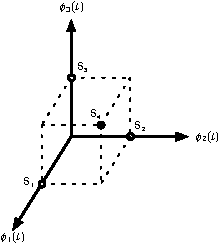
\includegraphics[width=4cm]{./Figuras/Problema4_5_sol}\end{figure*}}
\end{enumerate}
}
{

Every T seconds, a transmitter sends across an AWGN channel one of the four following equiprobable waveforms.
	
	\begin{displaymath}
		\begin{array}{l}
			s_1 (t)=\phi_1 (t) \\
			s_2 (t)=\phi_2 (t) \\
			s_3 (t)=\phi_3 (t) \\
			s_4 (t)=\phi_1 (t)+\phi_2 (t)+\phi_3 (t) 
		\end{array}
	\end{displaymath}

	\begin{displaymath}
		\phi_i(t) = \sqrt{\frac{2}{T}} cos(\omega_i t) 
	\end{displaymath}
	
	\begin{displaymath}
		\begin{array}{lll}
			0\leq t<T & \omega_i = \frac{2\pi i}{T} & i=1,2,3
		\end{array}
	\end{displaymath}
	
	\begin{enumerate}
		\item Explain whether or not the signals $\phi_i(t)$ constitute an orthonormal basis.
		\item Plot the constellation corresponding to this signal set.
	\end{enumerate}
}
{
\begin{enumerate}
	\item Yes, the signals constitute an orthonormal basis.
	\item \
	{\begin{figure*}[h!]\centering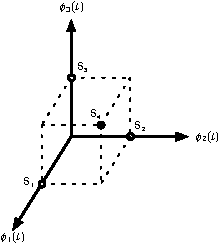
\includegraphics[width=4cm]{./Figuras/Problema4_5_sol}\end{figure*}}
\end{enumerate}
}

\newpage

%%%%%%%%%%%%%
% PROBLEMA 6
%%%%%%%%%%%%%
\Problema{

	Un sistema de transmisión de tipo binario utiliza las señales $s_0(t)$ y $s_1(t)$ para transmitir dos símbolos equiprobables, a través de un sistema que introduce ruido gaussiano cuya densidad espectral de potencia es  $N_0/2$.

\begin{displaymath}
	\begin{array}{ll}
		s_0(t) = A \cdot cos\left ( \frac{\pi t}{T} \right ) & 0\leq t<T \\
		s_1(t) = A \cdot cos\left ( \frac{\pi t}{T} + \phi \right ) & 0\leq t<T \\
	\end{array}
\end{displaymath}

Donde $T$ es la duración del símbolo.

\begin{enumerate}
	\item Calcular una base ortonormal para $s_0(t)$ y $s_1(t)$.
	\item Obtener la constelación correspondiente a las dos señales y representar las regiones de decisión.
	\item Determinar la probabilidad de error.
\end{enumerate}

}
{

\begin{enumerate}
	\item \begin{displaymath}
		\begin{array}{ll}
			\phi_1(t) = \sqrt{\frac{2}{T}} cos \left ( \frac{\pi t}{T} \right ) & 0 \leq t < T \\
			\phi_2(t) = -\sqrt{\frac{2}{T}} sen \left ( \frac{\pi t}{T} \right ) & 0 \leq t < T 
		\end{array}
		\end{displaymath}
	\item \begin{displaymath}
		\begin{array}{l}
			s_0(t) = A \sqrt{\frac{T}{2}} \cdot\phi_1(t) \\
			s_1(t) = A \sqrt{\frac{T}{2}} \cdot cos(\phi) \cdot \phi_1(t) + A \sqrt{\frac{T}{2}} \cdot sen(\phi) \cdot \phi_2(t)
		\end{array}
		\end{displaymath}
		Regiones de decisión: 
		\begin{itemize}
			\item 	$\frac{\phi}{2} < \theta < (\frac{\phi}{2} + \pi)$
			\item 	$(\frac{\phi}{2} + \pi) \leq \theta \leq \frac{\phi}{2}$  
		\end{itemize}
	\item $P_e = Q\left ( A \sqrt{\frac{T}{N_0}} sen \frac{\phi}{2} \right )$
\end{enumerate}

}
{

	A binary transmission system employs the signals $s_0(t)$ and $s_1(t)$ to transmit two equiprobable hypothesis, across a system affected by AWGN with power spectral density $N_0/2$.

\begin{displaymath}
	\begin{array}{ll}
		s_0(t) = A \cdot cos\left ( \frac{\pi t}{T} \right ) & 0\leq t<T \\
		s_1(t) = A \cdot cos\left ( \frac{\pi t}{T} + \phi \right ) & 0\leq t<T \\
	\end{array}
\end{displaymath}

where $T$ is the symbol period.

\begin{enumerate}
	\item Calculate an orthonormal basis for $s_0(t)$ and $s_1(t)$.
	\item Obtain the constellation corresponding to both signals and plot the decision regions.
	\item Calculate the error probability.
\end{enumerate}

}
{

\begin{enumerate}
	\item \begin{displaymath}
		\begin{array}{ll}
			\phi_1(t) = \sqrt{\frac{2}{T}} cos \left ( \frac{\pi t}{T} \right ) & 0 \leq t < T \\
			\phi_2(t) = -\sqrt{\frac{2}{T}} sen \left ( \frac{\pi t}{T} \right ) & 0 \leq t < T 
		\end{array}
		\end{displaymath}
	\item \begin{displaymath}
		\begin{array}{l}
			s_0(t) = A \sqrt{\frac{T}{2}} \cdot\phi_1(t) \\
			s_1(t) = A \sqrt{\frac{T}{2}} \cdot cos(\phi) \cdot \phi_1(t) + A \sqrt{\frac{T}{2}} \cdot \sin(\phi) \cdot \phi_2(t)
		\end{array}
		\end{displaymath}
		Decision regions: 
		\begin{itemize}
			\item 	$\frac{\phi}{2} < \theta < (\frac{\phi}{2} + \pi)$
			\item 	$(\frac{\phi}{2} + \pi) \leq \theta \leq \frac{\phi}{2}$  
		\end{itemize}
	\item $P_e = Q\left ( A \sqrt{\frac{T}{N_0}} sen \frac{\phi}{2} \right )$
\end{enumerate}

}

\newpage

%%%%%%%%%%%%%
% PROBLEMA 7
%%%%%%%%%%%%%
\Problema{
[Sept1999] Un sistema de comunicación transmite las señales $s_i(t)$, $i = 0,1,2,3,4,5,6,7$.

\begin{displaymath}
	\begin{array}{llll}
		s_i(t) = A \cdot cos \left ( \omega_c t + \frac{\pi}{4}i \right ) ; & 0 \leq t < T ; & \omega_c = n_c \cdot \frac{2\pi}{T} ; & n_c \in \mathbb{Z}
	\end{array}
\end{displaymath}

por un canal con ruido aditivo blanco gaussiano con densidad espectral de potencia de valor $N_0/2$ y media nula. Se pide:

\begin{enumerate}
	\item Obtener una base ortonormal para representar estas señales.
	\item Dibujar el esquema de bloques de un receptor de correlación diseñado para detectar estas señales.
	\item Calcular una cota superior de la probabilidad de error de símbolo en el caso de $A = 0.2 mV$, $N_0/2 = 10^{-15}  W/Hz$ y $T = 8 \mu s$.
\end{enumerate}

\textsc{Nota:} $P_e \leq (M-1) \cdot Q\left (\frac{d_{min}}{\sqrt{2N_0}} \right )$
}
{

\begin{enumerate}
	\item Base ortonormal:
		\begin{displaymath}
			\begin{array}{ll}
				\phi_1(t) = \sqrt{\frac{2}{T}} \cdot cos(\omega_c t) & \phi_2(t) = \sqrt{\frac{2}{T}} \cdot sen(\omega_c t)
			\end{array}
		\end{displaymath}
	\item Esquema:
		\begin{figure*}[h!]
			\centering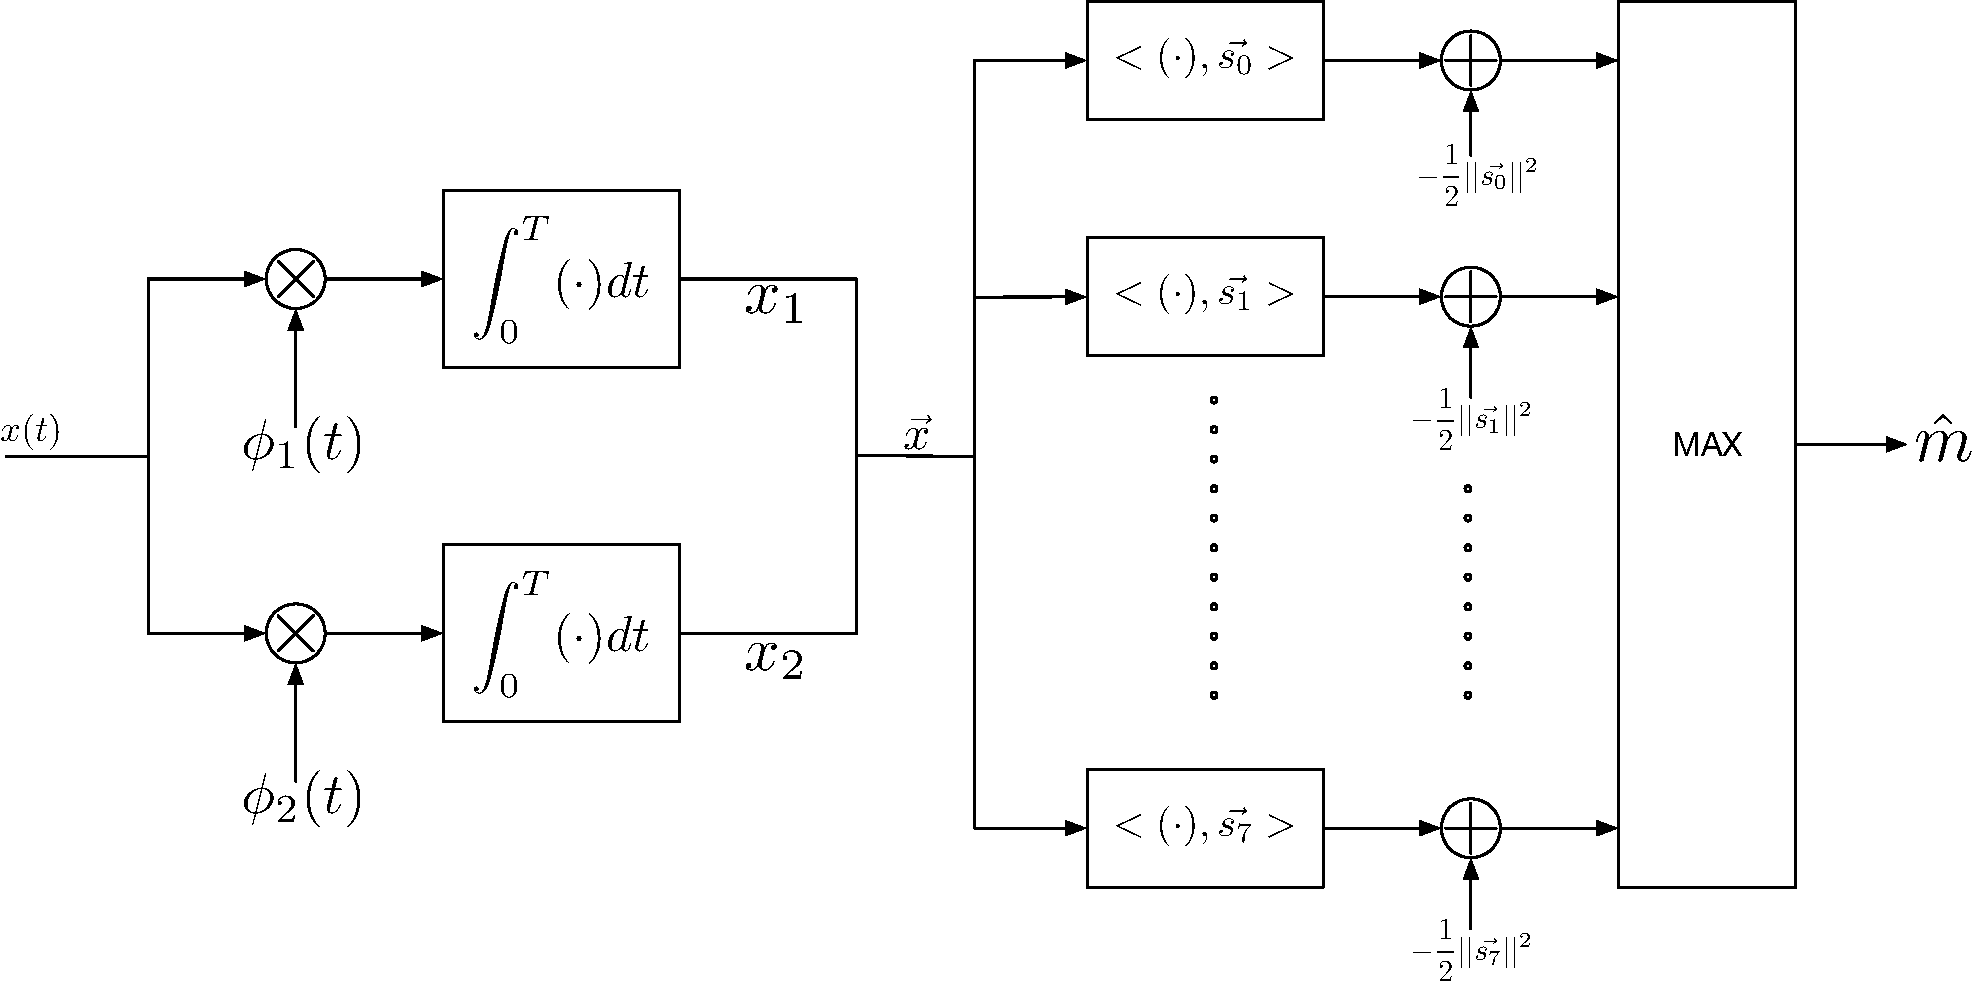
\includegraphics[width=12cm]{./Figuras/Problema4_7_sol}
		\end{figure*}
	\item $P_e \leq 5.55 \cdot 10^{-6}$
\end{enumerate}
}
{
[Sep1999] A communication system transmits the signals $s_i(t)$, $i = 0,1,2,3,4,5,6,7$.

\begin{displaymath}
	\begin{array}{llll}
		s_i(t) = A \cdot cos \left ( \omega_c t + \frac{\pi}{4}i \right ) ; & 0 \leq t < T ; & \omega_c = n_c \cdot \frac{2\pi}{T} ; & n_c \in \mathbb{Z}
	\end{array}
\end{displaymath}

across an AWGN channel with power spectral density $N_0/2$.

\begin{enumerate}
	\item Provide an orthonormal basis to represent these signals.
	\item Plot the general block diagram of a correlator receiver designed to detect these signals.
	\item Calculate an upper bound for the symbol error probability when we have the data $A = 0.2 mV$, $N_0/2 = 10^{-15}  W/Hz$ y $T = 8 \mu s$.
\end{enumerate}

\textsc{Note:} $P_e \leq (M-1) \cdot Q\left (\frac{d_{min}}{\sqrt{2N_0}} \right )$
}
{

\begin{enumerate}
	\item Orthonormal basis:
		\begin{displaymath}
			\begin{array}{ll}
				\phi_1(t) = \sqrt{\frac{2}{T}} \cdot cos(\omega_c t) & \phi_2(t) = \sqrt{\frac{2}{T}} \cdot sen(\omega_c t)
			\end{array}
		\end{displaymath}
	\item \
		\begin{figure*}[h!]
			\centering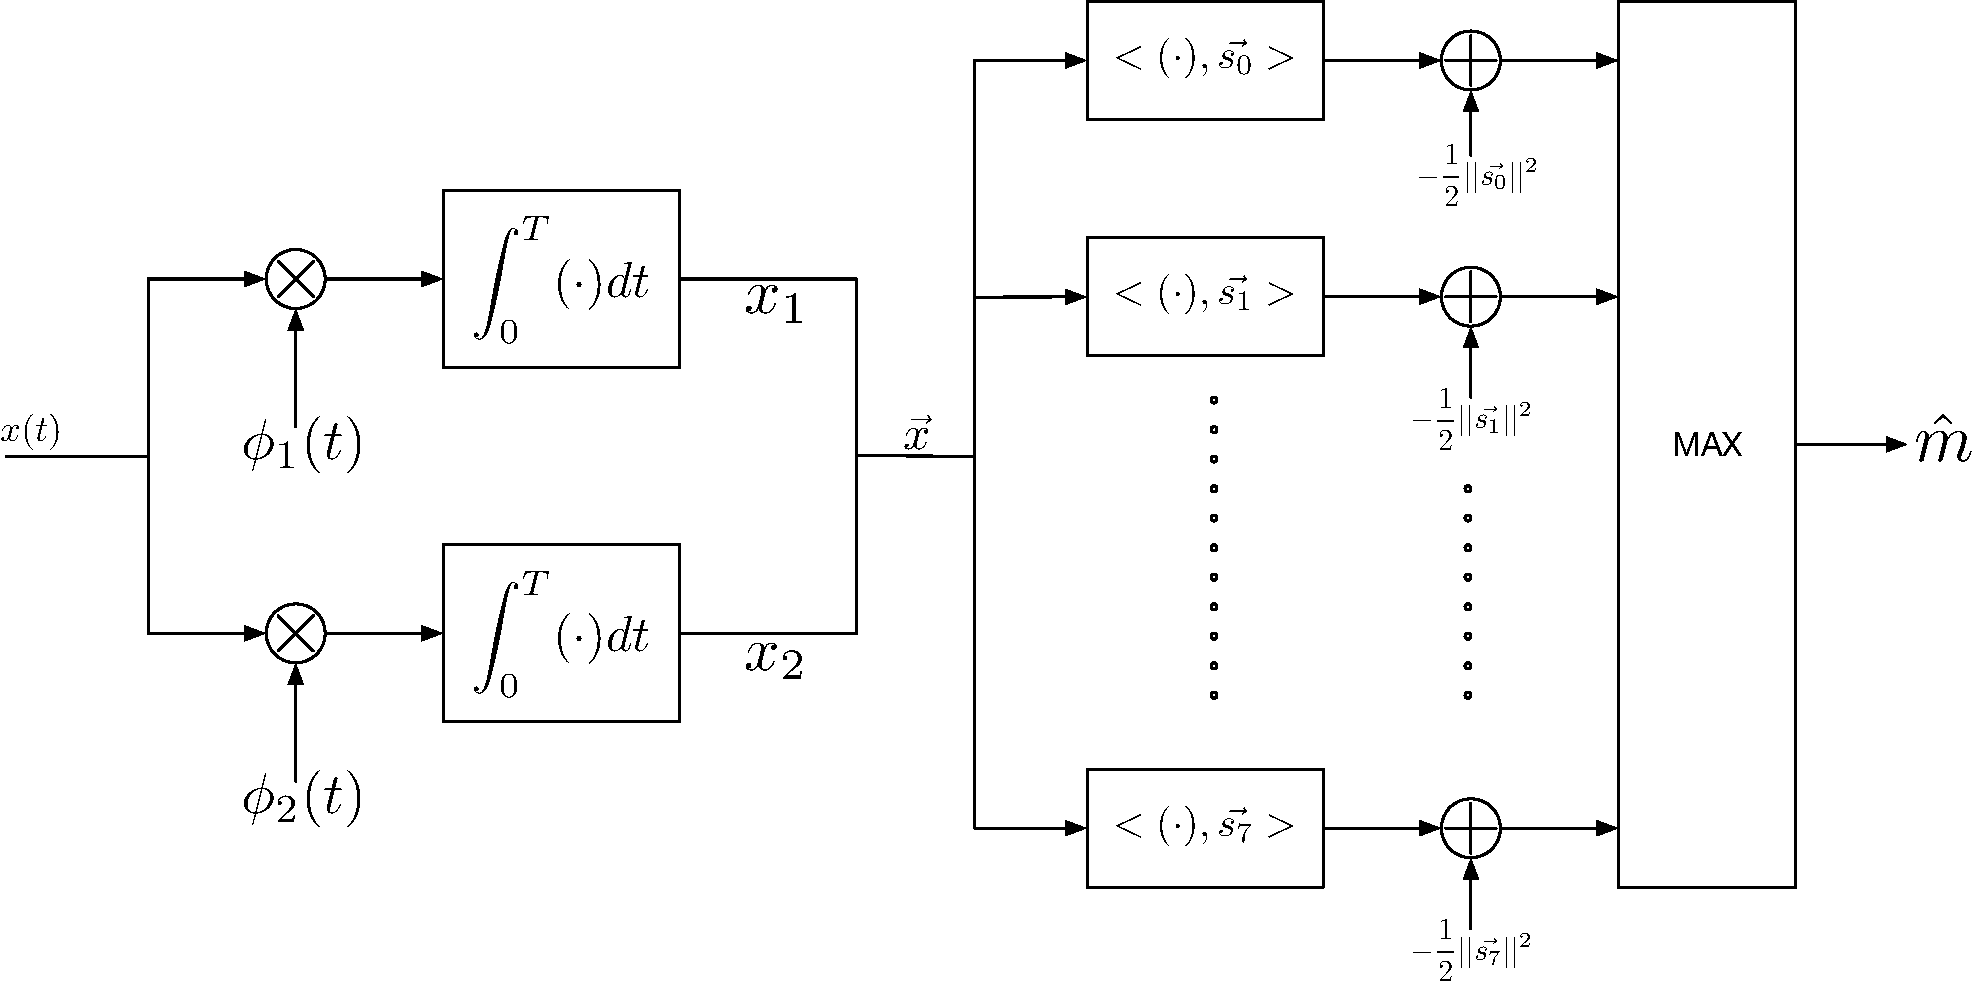
\includegraphics[width=12cm]{./Figuras/Problema4_7_sol}
		\end{figure*}
	\item $P_e \leq 5.55 \cdot 10^{-6}$
\end{enumerate}
}

\newpage

%%%%%%%%%%%%%
% PROBLEMA 8
%%%%%%%%%%%%%
\Problema{
[Junio1999] Las señales $s_i(t)$, $i=1,2,3,4$, se utilizan para transmitir cuatro mensajes equiprobables por un canal con ruido aditivo blanco gaussiano con densidad espectral de potencia de valor $N_0/2$. 
	\ \\
	
	\begin{tabular}[h!]{ll}
	$ s_1(t) = \left \{
		\begin{array}{ll}
			\frac{A}{2} & 0 \leq t <\frac{T}{2} \\
			& \\
			-\frac{A}{2} & \frac{T}{2} \leq t < T \\
		\end{array} \right.$
	&
	$ s_2(t) = \left \{
		\begin{array}{ll}
			-\frac{A}{2} & 0 \leq t <\frac{T}{2} \\
			& \\
			\frac{A}{2} & \frac{T}{2} \leq t < T \\
		\end{array} \right.$ \\
		& \\
	$ s_3(t) = \left \{
		\begin{array}{ll}
			\frac{3A}{2} & 0 \leq t <\frac{T}{2} \\
			& \\
			-\frac{3A}{2} & \frac{T}{2} \leq t < T \\
		\end{array} \right.$
	&
	$ s_1(t) = \left \{
		\begin{array}{ll}
			-\frac{3A}{2} & 0 \leq t <\frac{T}{2} \\
			& \\
			\frac{3A}{2} & \frac{T}{2} \leq t < T \\
		\end{array} \right.$
	\end{tabular}
	
	Se pide:
	
	\begin{enumerate}
		\item Obtener una base ortonormal para el espacio de señal e indicar cuál es su dimensión.
		\item Dibujar la constelación de señal con indicación de las regiones de decisión con el criterio de mínima probabilidad de error.
		\item Dibujar las respuestas al impulso de los filtros adaptados a cada una de las señales de la base.
		\item Calcular la probabilidad de error de símbolo en función de $A$ y de $N_0/2$.
	\end{enumerate}

}
{

\begin{enumerate}
	\item $\phi(t) = \left \{ \begin{array}{ll} \frac{1}{\sqrt{T}} & 0 \leq t < \frac{T}{2} \\  -\frac{1}{\sqrt{T}} & \frac{T}{2} \leq t < T \end{array} \right.$
	
	\item \ \\
	\begin{figure*}[h!] \centering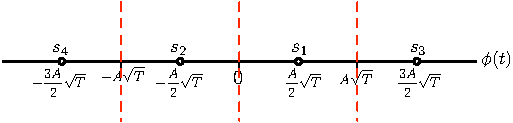
\includegraphics[width=8cm]{./Figuras/Problema4_8_sola}	\end{figure*}
	
	\ \\
	\ \\
	\item \ \\
	\begin{figure*}[h!] 	\centering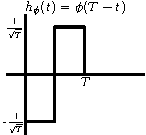
\includegraphics[width=3cm]{./Figuras/Problema4_8_solb} 	\end{figure*}
	
	\item $P_e = \frac{3}{2} Q \left ( A \sqrt{\frac{T}{2N_0}} \right ) $
	
\end{enumerate}

}
{
[June1999] The signals $s_i(t)$, $i=1,2,3,4$, are used to transmit four equiprobable messages across an AWGN channel with power spectral density $N_0/2$. 
	\ \\
	
	\begin{tabular}[h!]{ll}
	$ s_1(t) = \left \{
		\begin{array}{ll}
			\frac{A}{2} & 0 \leq t <\frac{T}{2} \\
			& \\
			-\frac{A}{2} & \frac{T}{2} \leq t < T \\
		\end{array} \right.$
	&
	$ s_2(t) = \left \{
		\begin{array}{ll}
			-\frac{A}{2} & 0 \leq t <\frac{T}{2} \\
			& \\
			\frac{A}{2} & \frac{T}{2} \leq t < T \\
		\end{array} \right.$ \\
		& \\
	$ s_3(t) = \left \{
		\begin{array}{ll}
			\frac{3A}{2} & 0 \leq t <\frac{T}{2} \\
			& \\
			-\frac{3A}{2} & \frac{T}{2} \leq t < T \\
		\end{array} \right.$
	&
	$ s_1(t) = \left \{
		\begin{array}{ll}
			-\frac{3A}{2} & 0 \leq t <\frac{T}{2} \\
			& \\
			\frac{3A}{2} & \frac{T}{2} \leq t < T \\
		\end{array} \right.$
	\end{tabular}
	\ \\
	\ \\
	\begin{enumerate}
		\item Obtain an orthonormal basis for the signal space considered and give its dimension.
		\item Plot the signal constellation and the decision regions corresponding to the criterion of minimum error probability.
		\item Plot the impulse responses of the matched filters corresponding to each of the basis signals.
		\item Calculate the symbol error probability as a function of $A$ and $N_0/2$.
	\end{enumerate}

}
{

\begin{enumerate}
	\item $\phi(t) = \left \{ \begin{array}{ll} \frac{1}{\sqrt{T}} & 0 \leq t < \frac{T}{2} \\  -\frac{1}{\sqrt{T}} & \frac{T}{2} \leq t < T \end{array} \right.$
	
	\item \ \\
	\begin{figure*}[h!] \centering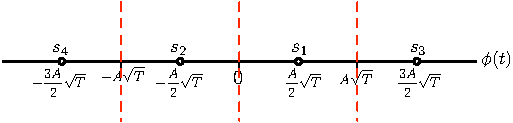
\includegraphics[width=8cm]{./Figuras/Problema4_8_sola}	\end{figure*}
	\ \\
	\ \\
	\ \\
	\item \ \\
	\ \\
	\begin{figure*}[h!] 	\centering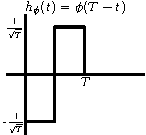
\includegraphics[width=4cm]{./Figuras/Problema4_8_solb} 	\end{figure*}
	
	\item $P_e = \frac{3}{2} Q \left ( A \sqrt{\frac{T}{2N_0}} \right ) $
\end{enumerate}

}
\newpage



\newpage

%%%%%%%%%%%%%
% PROBLEMA 10
%%%%%%%%%%%%%
\Problema{

	Un sistema de comunicación digital utiliza una de las siguientes señales para transmitir cada uno de los cuatro mensajes equiprobables siguientes:
	
	\begin{displaymath}
		\begin{array}{l}
			s_1(t) = 0 \\
			s_2(t) = sen \left ( \omega_0 t \right ) \\
			s_3(t) = cos \left ( \omega_0 t \right ) \\
			s_4(t) = \sqrt{2} \cdot sen \left ( \omega_0 t + \frac{\pi}{4} \right )
		\end{array}
	\end{displaymath}
	
	donde $0 \leq t < T$ y $\omega_0 = n \cdot \frac{2\pi}{T}$ con $n \in \mathbb{Z}$.

	\begin{enumerate}
		\item Obtener una base ortonormal que permita representar el conjunto de señales.
		\item Obtener los coeficientes correspondientes a cada una de las señales y dibujar la constelación correspondiente.
		\item Calcular la cota simplificada de la probabilidad media de error de símbolo en el caso de $N_0/2=10^{-11} W/Hz$ y $T=0.8 ns$.
	\end{enumerate}
	

}
{

\begin{enumerate}
	\item \
	\begin{displaymath}
		\begin{array}{ll}
			\phi_1(t) = \sqrt{\frac{2}{T}} cos \left ( \omega_0 t  \right ) & 0 \leq t < T \\
			\phi_2(t) = \sqrt{\frac{2}{T}} sen \left ( \omega_0 t  \right ) & 0 \leq t < T \\
		\end{array}
	\end{displaymath}
	\item \
	\begin{displaymath}
		\begin{array}{ll}
			\bar{s_1} = \left [0, 0 \right ] & \bar{s_2} = \left [0, \sqrt{\frac{T}{2}} \right ] \\
			\bar{s_3} = \left [\sqrt{\frac{T}{2}}, 0 \right ] & \bar{s_4} = \left [\sqrt{\frac{T}{2}}, \sqrt{\frac{T}{2}} \right ]\\
		\end{array}
	\end{displaymath}
	\item $P_e \leq 2.902 \cdot 10^{-3}$
\end{enumerate}
}
{

	A digital communication system uses the following signals to transmit four equiprobable symbols:
	
	\begin{displaymath}
		\begin{array}{l}
			s_1(t) = 0 \\
			s_2(t) = sen \left ( \omega_0 t \right ) \\
			s_3(t) = cos \left ( \omega_0 t \right ) \\
			s_4(t) = \sqrt{2} \cdot sen \left ( \omega_0 t + \frac{\pi}{4} \right )
		\end{array}
	\end{displaymath}
	
	where $0 \leq t < T$ and $\omega_0 = n \cdot \frac{2\pi}{T}$ with $n \in \mathbb{Z}$.

	\begin{enumerate}
		\item Obtain an orthonormal basis set to represent the given signals.
		\item Obtain the signal vectors for each of the signals $s_i(t)$ and plot the constellation.
		\item Calculate the simplified union bound of the probability of symbol error knowing that $N_0/2=10^{-11} W/Hz$ and $T=0.8 ns$.
	\end{enumerate}
	
}
{

\begin{enumerate}
	\item \
	\begin{displaymath}
		\begin{array}{ll}
			\phi_1(t) = \sqrt{\frac{2}{T}} cos \left ( \omega_0 t  \right ) & 0 \leq t < T \\
			\phi_2(t) = \sqrt{\frac{2}{T}} sen \left ( \omega_0 t  \right ) & 0 \leq t < T \\
		\end{array}
	\end{displaymath}
	\item \
	\begin{displaymath}
		\begin{array}{ll}
			\bar{s_1} = \left [0, 0 \right ] & \bar{s_2} = \left [0, \sqrt{\frac{T}{2}} \right ] \\
			\bar{s_3} = \left [\sqrt{\frac{T}{2}}, 0 \right ] & \bar{s_4} = \left [\sqrt{\frac{T}{2}}, \sqrt{\frac{T}{2}} \right ]\\
		\end{array}
	\end{displaymath}
	\item $P_e \leq 2.902 \cdot 10^{-3}$
\end{enumerate}
}

\newpage

%%%%%%%%%%%%%
% PROBLEMA 11
%%%%%%%%%%%%%
\Problema{

	Dadas las tres señales de la siguiente figura, correspondientes a la transmisión de tres símbolos equiprobables, se pide: 
 
 \begin{figure*}[h!] 	\centering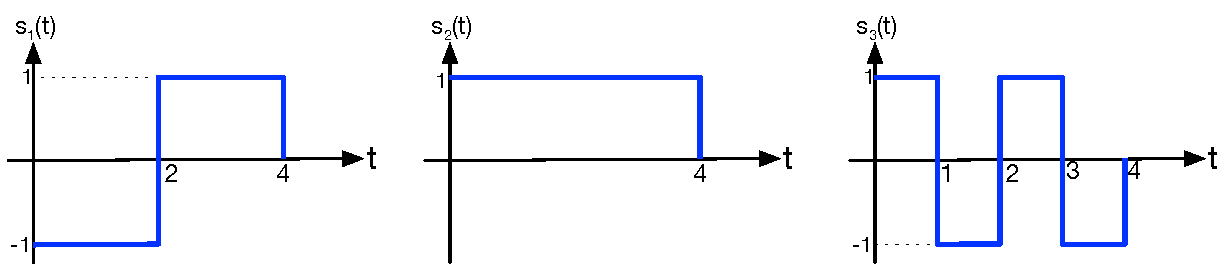
\includegraphics[width=12cm]{./Figuras/Problema4_11a} 	\end{figure*}
	
	\begin{enumerate}
		\item Obtener una base ortonormal que permita representar las tres señales. 
		\item Representar la constelación correspondiente a las tres señales.
		\item Acotar el valor de la probabilidad de error, sabiendo que el canal introduce ruido blanco gaussiano cuya densidad espectral de potencia vale $N_0/2 = 10^{-2} W/Hz$. 
		\item Expresar la señal $x(t)$ representada en la siguiente figura en función de la base ortonormal anterior y representarla en la constelación.
		\\
		\begin{tabular}{lr}
			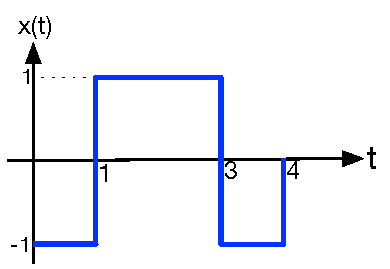
\includegraphics[width=5cm]{./Figuras/Problema4_11b} &
			\begin{math}
			x(t) = \left\{ \begin{array}{ll} -1 & 0\leq t < 1 \\ 1 & 1 \leq t < 3  \\ 1 & 3 \leq t < 4 \end{array} \right. 
			\end{math}  \\
		\end{tabular}
		\item Indicar, justificadamente, por cuál de los tres símbolos se decantaría el receptor si se recibiese la señal $x(t)$.
	\end{enumerate}

}
{
\begin{enumerate}
	\item $\phi_i(t) = \frac{1}{2} \cdot s_i(t) \,\, ; \, \, i=1,2,3$

	\item \ \\
	
	\begin{figure*}[h!] 	\centering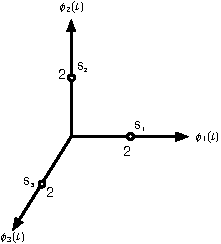
\includegraphics[width=3cm]{./Figuras/Problema4_11_sol} 	\end{figure*}

	\item $P_e \leq 2 \cdot Q(14.14)$
	\item $\bar{x} = [0,0,0]$. Cogería uno al azar.
\end{enumerate}
}
{

	The following signals are used to send three equiprobable symbols: 
 
 \begin{figure*}[h!] 	\centering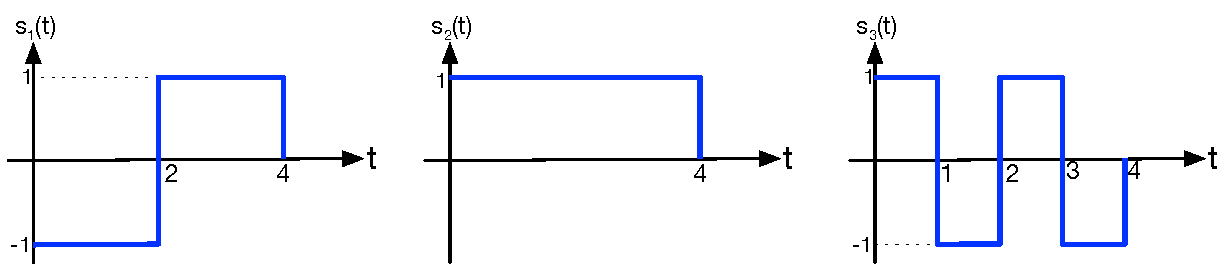
\includegraphics[width=12cm]{./Figuras/Problema4_11a} 	\end{figure*}
	
	\begin{enumerate}
		\item Obtain an orthonormal basis set to represent the given signals. 
		\item Plot the signals in the signal space. 
		\item Provide a bound on the probability of error knowing that the AWGN channel is characterized by a power spectral density of $N_0/2 = 10^{-2}  W/Hz$. 
		\item Use the set of basis obtained in a. to represent the following signal $x(t)$ and plot it in the constellation. 
				\\
		\begin{tabular}{lr}
			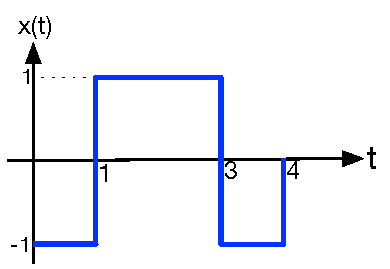
\includegraphics[width=5cm]{./Figuras/Problema4_11b} &
			\begin{math}
			x(t) = \left\{ \begin{array}{ll} -1 & 0\leq t < 1 \\ 1 & 1 \leq t < 3  \\ 1 & 3 \leq t < 4 \end{array} \right. 
			\end{math}  \\
		\end{tabular}
		\item Suppose that signal $x(t)$ is received. Justify which symbol would the receiver detect in this case. 
	\end{enumerate}

}
{
\begin{enumerate}
	\item $\phi_i(t) = \frac{1}{2} \cdot s_i(t) \,\, ; \, \, i=1,2,3$
	
	\item \ \\
	\begin{figure*}[h!] 	\centering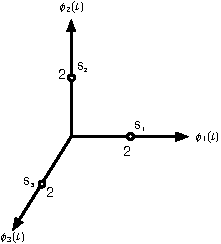
\includegraphics[width=3cm]{./Figuras/Problema4_11_sol} 	\end{figure*}
	\item $P_e \leq 2 \cdot Q(14.14)$
	\item $\bar{x} = [0,0,0]$. It will randomly choose one symbol.
\end{enumerate}
}


\Problema{
	[Junio2001] Dadas las dos constelaciones de la figura, donde las señales de la base son:

	\begin{displaymath}
		\phi_1(t) = \left \{ \begin{array}{ll} \sqrt{\frac{2}{T}} \cos \left ( \frac{2\pi}{T} t \right ) & 0\leq t < T \\ 0 & c.c. \end{array} \right .
	\end{displaymath}
	\begin{displaymath}
		\phi_2(t) = \left \{ \begin{array}{ll} \sqrt{\frac{2}{T}} \sen \left ( \frac{2\pi}{T} t \right ) & 0\leq t < T \\ 0 & c.c. \end{array} \right .
	\end{displaymath}

	se pide:

	\begin{enumerate}
		\item Obtener las expresiones temporales de la señales de las dos constelaciones.
  \item Obtener la energía media transmitida por símbolo ($E_s$) en cada una de las dos constelaciones.
  \item Calcular la cota de la unión de la probabilidad de error de símbolo en función de $E_s/N_0$ en las dos constelaciones.
	\end{enumerate}

	\begin{center}
		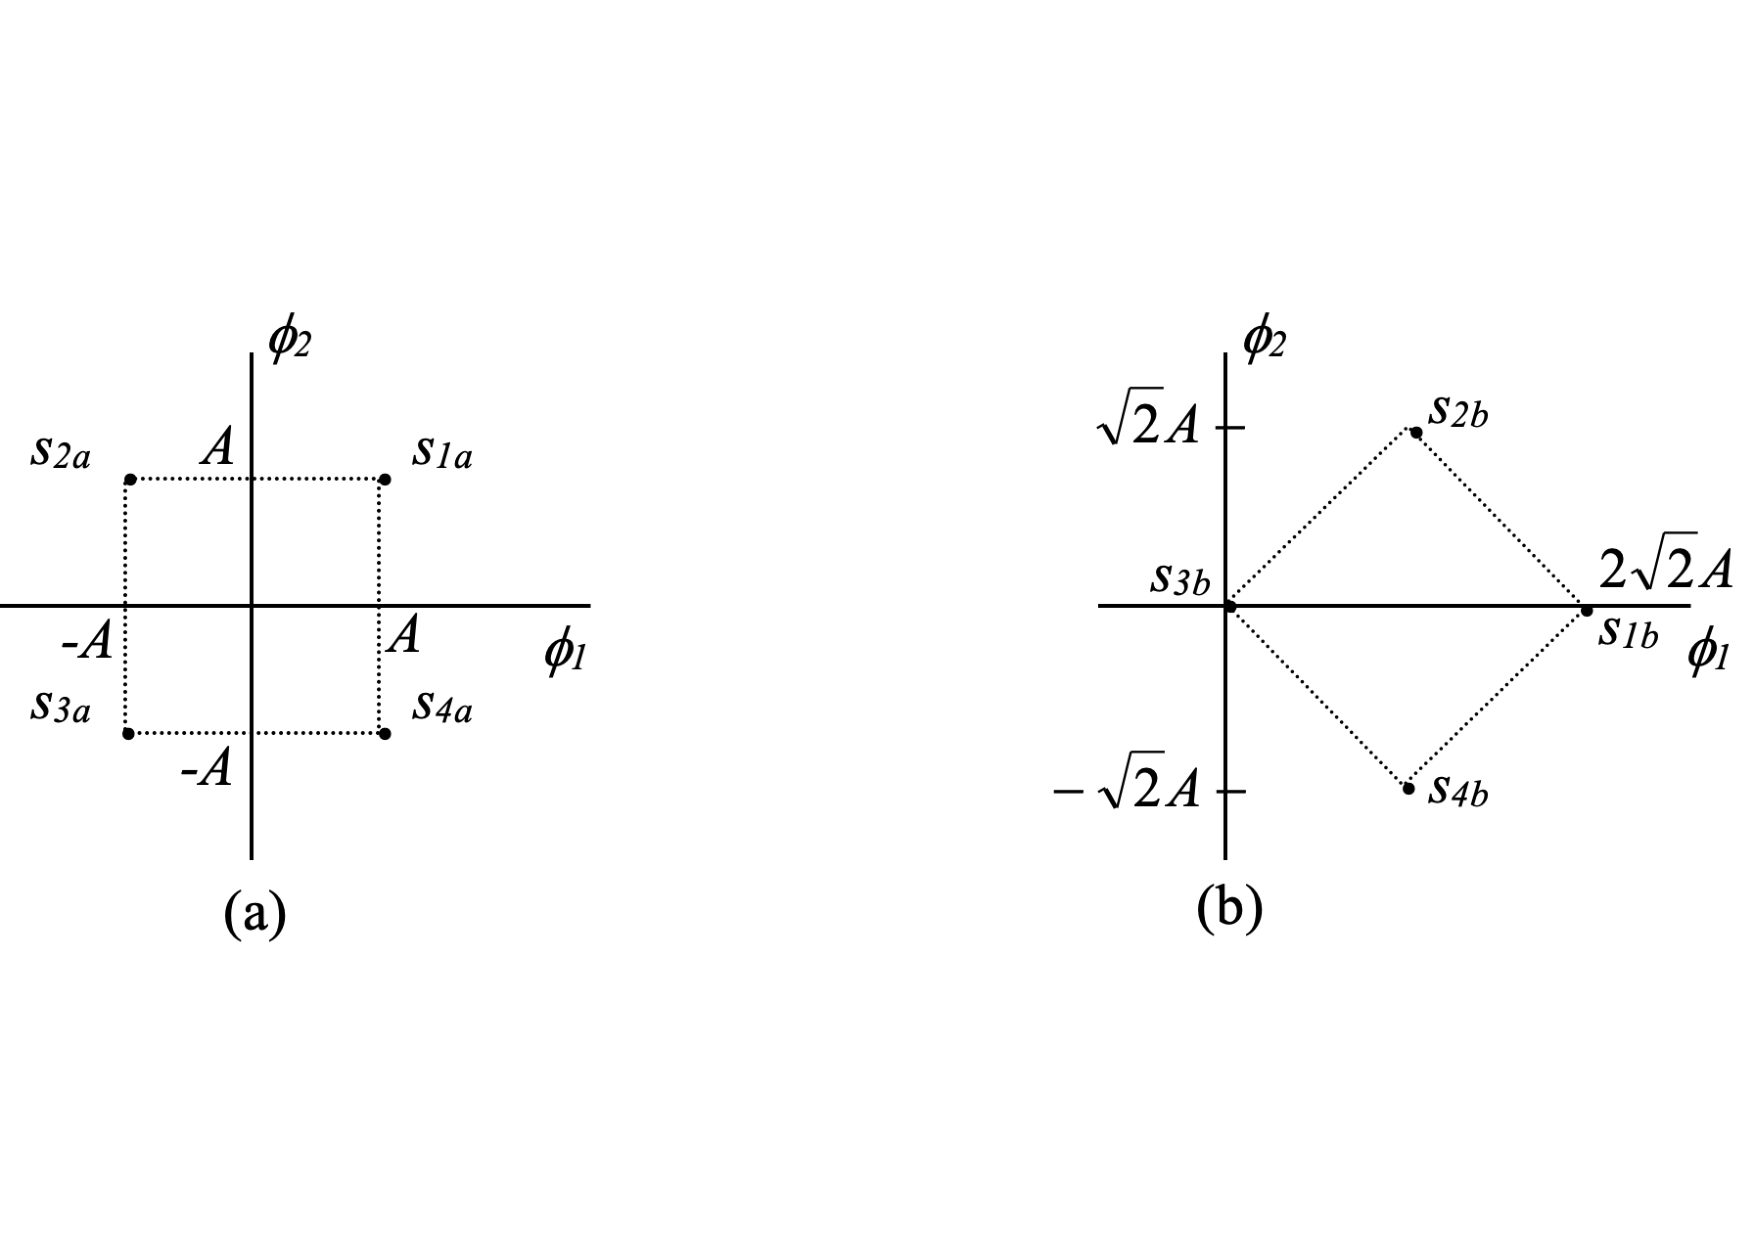
\includegraphics[width=12cm]{Figuras/Problema2001}
	\end{center}
}
{
	\begin{enumerate}
		\item $s_{1a}(t) = A \cdot \phi_1(t) + A \cdot \phi_2(t)$ \\
		$s_{2a}(t) = -A \cdot \phi_1(t) + A \cdot \phi_2(t)$ \\
		$s_{3a}(t) = -A \cdot \phi_1(t) - A \cdot \phi_2(t)$ \\
		$s_{4a}(t) = A \cdot \phi_1(t) - A \cdot \phi_2(t)$ \\
		$s_{1b}(t) = 2\sqrt{2}A \cdot \phi_1(t)$ \\
		$s_{2b}(t) = \sqrt{2} A \cdot \phi_1(t) + \sqrt{2} A \cdot \phi_2(t)$ \\
		$s_{3b}(t) = 0$ \\
		$s_{4b}(t) = \sqrt{2} A \cdot \phi_1(t) - \sqrt{2} A \cdot \phi_2(t)$ \\

		\item $P_e \leq 2 Q\left ( \frac{\sqrt{2}A}{\sqrt{N_0}} \right ) + Q \left ( \frac{2A}{\sqrt{N_0}} \right )$
  
		\item $E_{sa} = 2A^2$ \\
				$E_{sb} = 4A^2$
	\end{enumerate} 
}
{
	[June2001] Given the two constellations in the figure, where the base signals are:
		\begin{displaymath}
		\phi_1(t) = \left \{ \begin{array}{ll} \sqrt{\frac{2}{T}} \cos \left ( \frac{2\pi}{T} t \right ) & 0\leq t < T \\ 0 & c.c. \end{array} \right .
		\end{displaymath}
		\begin{displaymath}
		\phi_2(t) = \left \{ \begin{array}{ll} \sqrt{\frac{2}{T}} \sin \left ( \frac{2\pi}{T} t \right ) & 0\leq t < T \\ 0 & c.c. \end{array} \right .
		\end{displaymath}

		\begin{enumerate}
			\item Obtain the temporal expressions of the signals of the two constellations.
			   \item Obtain the average energy transmitted per symbol ($E_s$) in each of the two constellations.
			   \item Compute the union bound of the symbol error probability as a function of $E_s/N_0$ in the two constellations.
			\end{enumerate}

			\begin{center}
				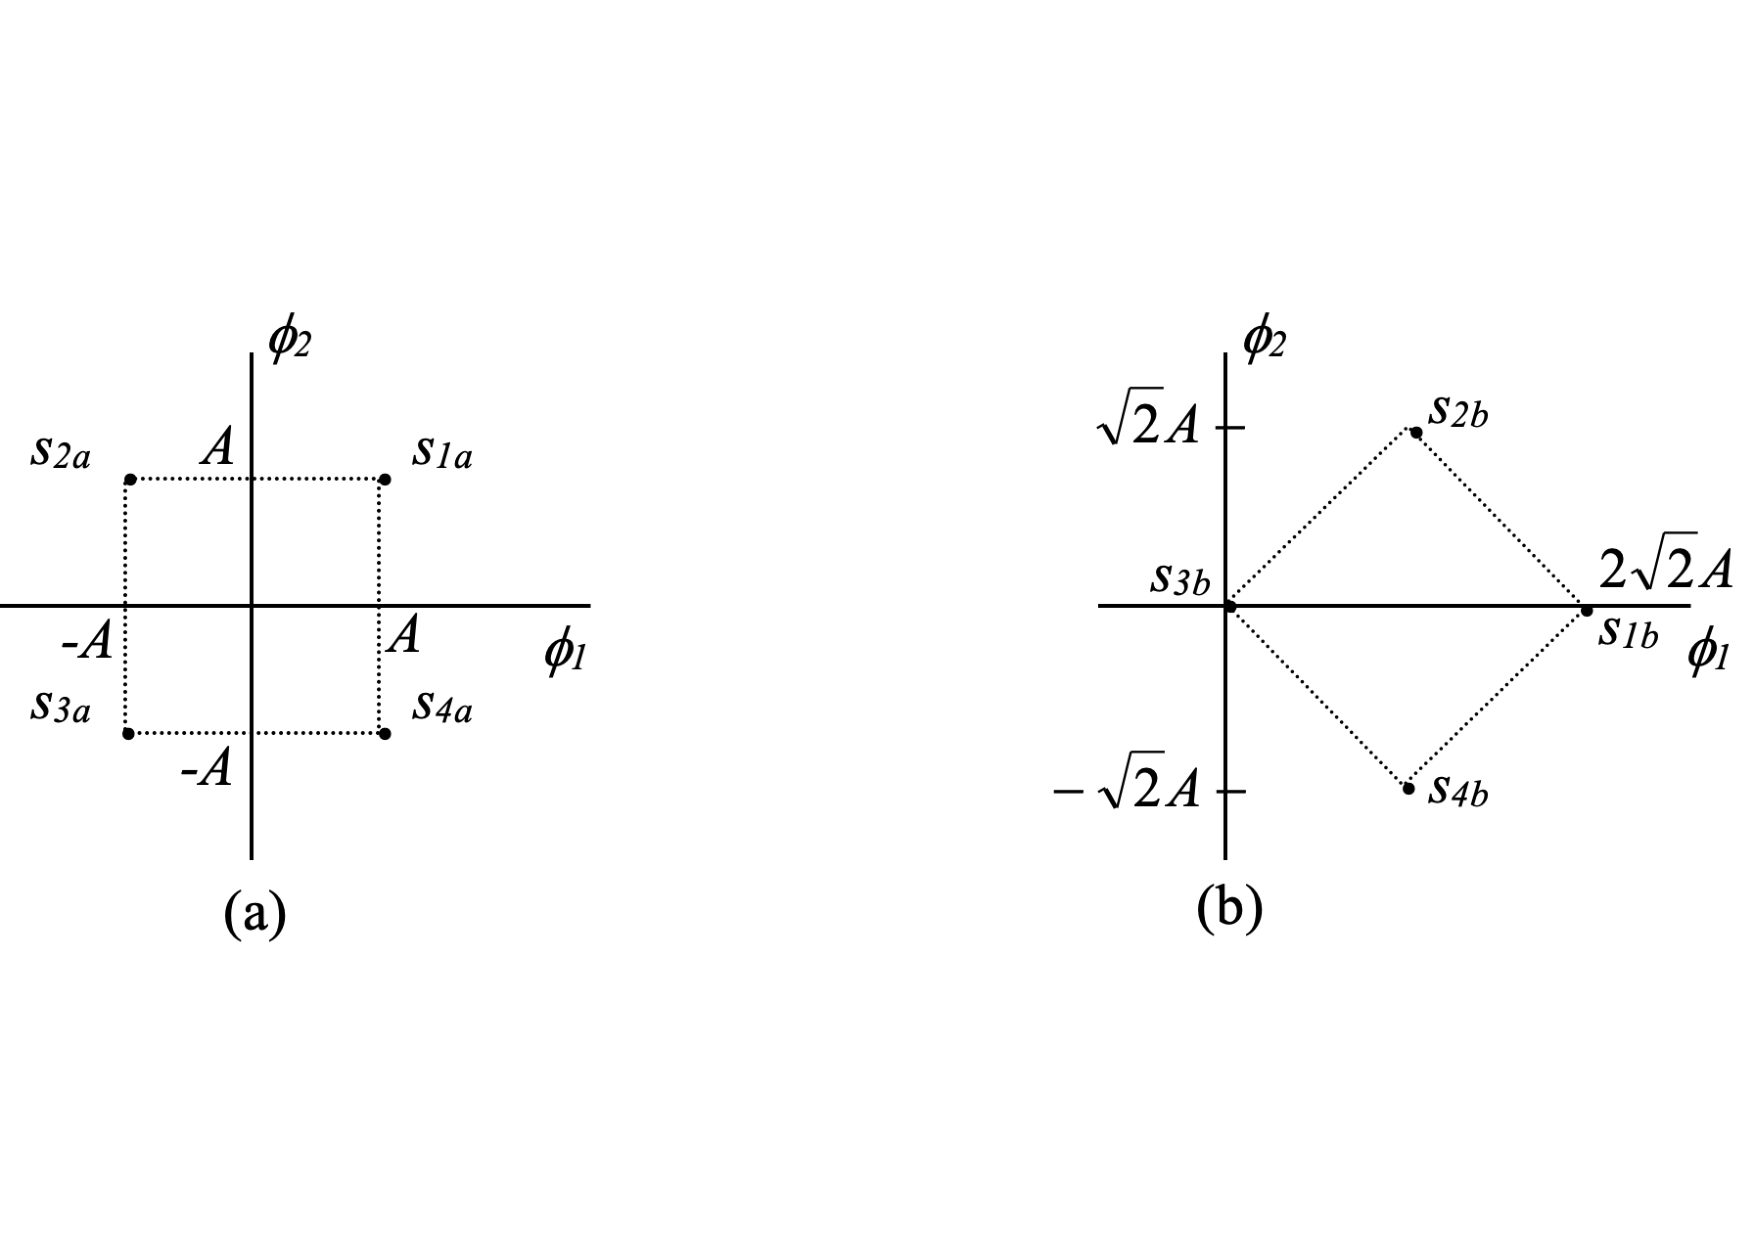
\includegraphics[width=12cm]{Figuras/Problema2001}
			\end{center}
}
{
	\begin{enumerate}
		\item $s_{1a}(t) = A \cdot \phi_1(t) + A \cdot \phi_2(t)$ \\
		$s_{2a}(t) = -A \cdot \phi_1(t) + A \cdot \phi_2(t)$ \\
		$s_{3a}(t) = -A \cdot \phi_1(t) - A \cdot \phi_2(t)$ \\
		$s_{4a}(t) = A \cdot \phi_1(t) - A \cdot \phi_2(t)$ \\
		$s_{1b}(t) = 2\sqrt{2}A \cdot \phi_1(t)$ \\
		$s_{2b}(t) = \sqrt{2} A \cdot \phi_1(t) + \sqrt{2} A \cdot \phi_2(t)$ \\
		$s_{3b}(t) = 0$ \\
		$s_{4b}(t) = \sqrt{2} A \cdot \phi_1(t) - \sqrt{2} A \cdot \phi_2(t)$ \\

		\item $P_e \leq 2 Q\left ( \frac{\sqrt{2}A}{\sqrt{N_0}} \right ) + Q \left ( \frac{2A}{\sqrt{N_0}} \right )$
  
		\item $E_{sa} = 2A^2$ \\
				$E_{sb} = 4A^2$
	\end{enumerate} 
}


\Problema{
	[Junio2003] Un sistema de comunicación digital transmite cada $T$ segundos una señal escogida de modo equiprobable entre los elementos del conjunto $\{s_i(t)\}, i=1,2,3$. Se pide:

	\begin{enumerate}
		\item Obtener una base ortonormal para representar $\{s_i(t)\}$.
  		\item Calcular la energía de cada una de las señales.
    	\item Dibujar la constelación de señal, con indicación expresa de las coordenadas de cada punto de señal.
     \item Calcular la cota de la unión simplificada de la probabilidad de error en función de la energía media de símbolo, $E_s$, para un canal de ruido blanco gaussiano aditivo con media nula y densidad espectral de potencia $N_0$ W/Hz cuando se utiliza un receptor de correlación.
	\end{enumerate}


	\begin{displaymath}
		s_1(t) = \left \{ \begin{array}{ll} 1 & 0\leq t < T \\ 0 & c.c. \end{array} \right .
	\end{displaymath}
	\begin{displaymath}
		s_2(t) = \left \{ \begin{array}{ll} -\cos\left ( \frac{\pi}{T}t \right ) & 0\leq t < T \\ 0 & c.c. \end{array} \right .
	\end{displaymath}
	\begin{displaymath}
		s_3(t) = \left \{ \begin{array}{ll} \cos^2 \left ( \frac{\pi}{2T}t \right ) & 0\leq t < T \\ 0 & c.c. \end{array} \right .
	\end{displaymath}
}
{
	\begin{enumerate}
		\item $\phi_1(t) = \frac{s_1(t)}{\sqrt{T}}$ \\
				$\phi_2(t) = \sqrt{\frac{2}{T}}s_2(t)$\\
		\item $E_1=T$, $E_2 = \frac{T}{2}$, $E_3 = \frac{3T}{8}$\\
				$E_s = \frac{5T}{8}$
		\item $\bar{s_1} = (\sqrt{T},0)$ \\
		$\bar{s_2} = (0, \sqrt{\frac{T}{2}})$ \\
		$\bar{s_3} = (\frac{\sqrt{T}}{2},-\frac{1}{2}\sqrt{\frac{T}{2}})$ \\
		\item $P_e \leq 2Q \left ( \sqrt{\frac{3 E_s}{10 N_0}} \right )$
	\end{enumerate}
}
{
	[June2003] A digital communication system transmits every $T$ seconds a signal chosen in an equiprobable way among the elements of the set $\{s_i(t)\}, i=1,2,3$. It is requested:

\begin{enumerate}
	\item Get an orthonormal basis to represent $\{s_i(t)\}$.
   	\item Calculate the energy of each of the signals.
    \item Draw the signal constellation, expressly indicating the coordinates of each signal point.
    \item Compute the simplified union bound of the error probability as a function of the mean symbol energy, $E_s$, for an additive Gaussian white noise channel with zero mean and power spectral density $N_0$ W/Hz when a correlation receiver is used.
\end{enumerate}

\begin{displaymath}
	s_1(t) = \left \{ \begin{array}{ll} 1 & 0\leq t < T \\ 0 & c.c. \end{array} \right .
\end{displaymath}
\begin{displaymath}
	s_2(t) = \left \{ \begin{array}{ll} -\cos\left ( \frac{\pi}{T}t \right ) & 0\leq t < T \\ 0 & c.c. \end{array} \right .
\end{displaymath}
\begin{displaymath}
	s_3(t) = \left \{ \begin{array}{ll} \cos^2 \left ( \frac{\pi}{2T}t \right ) & 0\leq t < T \\ 0 & c.c. \end{array} \right .
\end{displaymath}

}
{
	\begin{enumerate}
		\item $\phi_1(t) = \frac{s_1(t)}{\sqrt{T}}$ \\
				$\phi_2(t) = \sqrt{\frac{2}{T}}s_2(t)$\\
		\item $E_1=T$, $E_2 = \frac{T}{2}$, $E_3 = \frac{3T}{8}$\\
				$E_s = \frac{5T}{8}$
		\item $\bar{s_1} = (\sqrt{T},0)$ \\
		$\bar{s_2} = (0, \sqrt{\frac{T}{2}})$ \\
		$\bar{s_3} = (\frac{\sqrt{T}}{2},-\frac{1}{2}\sqrt{\frac{T}{2}})$ \\
		\item $P_e \leq 2Q \left ( \sqrt{\frac{3 E_s}{10 N_0}} \right )$
	\end{enumerate}
}


\begin{thebibliography}{100}
	\bibitem[Artés2012]{Artes} Antonio Artés et al. Comunicaciones Digitales. \url{http://www.tsc.uc3m.es/∼antonio/libro_comunicaciones}.
	\bibitem[Sklar2001]{Sklar} Bernard Sklar. Digital Communications 2nd Ed. Pearson, 2001.
	\end{thebibliography}
	
	


\end{document}



	
